\section{Introduction}
\subsection{Background and engineering problem}
GPU sharing for inference is an operating-system resource-management problem: several services compete for finite execution capacity, device memory and access to a runtime that may not expose the control required by a service-level objective. Increasing concurrent execution can improve aggregate work completed while worsening the response of an individual service. Conversely, reserving the entire accelerator for one model can simplify interference management but leaves less opportunity to use spare capacity. The engineering question is therefore conditional: which mechanism should be selected for a particular workload, latency objective, memory requirement and isolation boundary?

The evidence makes this tension concrete. The ParvaGPU manuscript reports a local configuration in which throughput increases from 354 to 446 requests/s as the number of MPS processes rises from one to three, while reported latency increases from 11 to 27 ms. These outcomes move in opposite desirable directions. The latency quantile is unspecified, so the example cannot establish a P99 service guarantee. XSched instead reports a foreground P99 ratio of 1.07 relative to standalone execution, compared with 1.53 for native Triton in the recorded configuration. These are different engineering objectives, not numbers on one ranking scale \cite{P011,P015}.

\subsection{Scope and contribution}
The unit of technical interpretation is concurrent inference on one physical GPU. A multi-GPU or cluster paper contributes only where a local sharing result can be separated from fleet scheduling. Mixed inference/training papers contribute inference outcomes and the associated background-work cost. Training throughput is not relabeled as inference throughput. Non-GPU accelerator results in otherwise relevant papers are outside the primary comparison.

This first draft synthesizes the supplied bounded corpus of 20 studies represented by 21 reports. Its contribution is a decision-oriented comparison that joins mechanisms, evaluation conditions, reported outcomes, implementation costs and limitations. It distinguishes performance interference, resource partitioning, memory protection and fault containment. It also retains adverse outcomes rather than selecting only favorable headline speedups.

The review is not an exhaustive census of the search results. The supplied record contains 559 retained records that were not advanced to source assessment. The first draft therefore supports candidate selection under observed conditions, while leaving the wider coverage question open. This boundary is part of the research method and must remain visible in the abstract, selection accounting and recommendations.

\subsection{Objectives}
The objectives are to classify the available mechanisms by their actual control boundaries; determine which outcomes are comparable; explain the conditions behind benefits and regressions; and derive recommendations that identify both expected benefit and sacrifice. The review does not seek a universal winning system. It seeks an auditable reason for choosing a candidate under stated constraints.

\section{Research questions}
The following research questions reproduce the submitted Task 1 protocol (Table 3).
\begin{description}
\item[RQ1] What time-slicing, MPS, MIG and API remoting mechanisms are evaluated for concurrent inference on one GPU, and how do sharing granularity, layer and isolation boundary classify them?
\item[RQ2] How do studies measure utilization, throughput, density, average/tail latency, predictability and interference, and how comparable are their experimental methods?
\item[RQ3] Under what GPU, workload, batch, tenant mix and configuration conditions are changes in utilization, throughput, density and latency reported?
\item[RQ4] What resource and fault isolation properties, trade-offs, implementation costs and conflicting results are reported, and what limits the evidence?
\item[RQ5] Which approach or combination is supported for specified inference-serving conditions and priorities, with what confidence and alternatives?
\end{description}

\section{Research methodology}
\subsection{Protocol and implemented method}
The submitted Task 1 protocol is preserved unchanged in the repository. It specifies independent screening and appraisal, stable record/report/study identifiers, page-level extraction and a condition-aware narrative synthesis. This draft follows its conceptual comparison rules while explicitly reporting deviations in execution. PRISMA supplies the reporting framework, while the search audit preserves the executed queries rather than replacing them with planned expressions \cite{prisma,prismas,kitchenham}.

The supplied Task 2 workbook is the source of the current corpus and historical decisions. GitHub's preceding status described an earlier 15-form assessment. Importing the newer workbook does not mean those older registers were silently rewritten. Task 3 stores the uploaded baseline separately and keeps the inherited research history available.

The implemented review used a single consolidated AI-assisted assessment under team direction. The uploaded materials refer to team checking, but contain no named independent item-level votes or signed verification record. This draft therefore does not claim completion of the protocol's independent second review or report inter-rater agreement. New activity logs identify the AI assistant's actions and actual checkpoint times. Historical batch or workbook-build times are not evidence of when a person screened a particular record.

\subsection{Source review of seven assigned studies}
A subsequent AI-assisted source review under Raazia's direction checked the accessed full text of S008--S014, their 70 appraisal items and 13 reported outcomes. It corrected Clockwork PDF anchors and added its reported TVM v0.7 environment detail, separated Torpor's evaluated sharing mode from its runtime-isolation design and deployment, and clarified the two-stage request-rate setup of KRYPTON's QoS experiment. All 13 retained numerical values were found in the accessed sources; the changes concern interpretation, source anchors and appraisal rationale. The original forms are preserved, and the active workbook records original and reviewed QA scores separately.

Under the submitted claim-specific rubric, Clockwork's and StreamBox's Q4 and Q9 scores each rise from 1 to 2: hardware/software/workload information and explicitly delimited performance/trust boundaries are reported. The seven-study QA sum changes from 110/140 to 114/140. This is a reporting appraisal, not a new performance result or an independent human vote. ParvaGPU's numerical checks remain specific to the accessed arXiv v1 manuscript. The remainder of the corpus is outside this seven-study source-review pass.

\subsection{Databases, search fields and period}
The active occurrence register represents ACM Digital Library, IEEE Xplore, Springer Nature Link and ScienceDirect, with supplementary named-paper lookups recorded separately. Their relevance is complementary: systems conferences, parallel/distributed systems research and journal literature provide different routes to sharing mechanisms. However, representation in an imported register is not equivalent to verified complete coverage of every planned database run.

The main publication window is 2020 through the date of each executed search in October 2026. IEEE and Springer entries record 11 October; ACM and ScienceDirect entries record 14 October. Later retrieval of a paper does not change an earlier search cutoff. The older journal survey used as an organizational benchmark is contextual literature, not an additional included primary study.

The executed expressions generally combine GPU terms, inference/model-serving terms and mechanism terms. Some interfaces use broad indexed fields rather than title/abstract/keywords. Broad fields can retrieve papers in which sharing terminology occurs only in references or background. Conversely, restricted inference expressions can miss papers described only as LLM serving. The exact retained expressions, fields and filters are reproduced in Appendix~\ref{app:search}; the workbook holds filenames and provenance.

The historical ACM master record contains displayed, claimed and parsed totals of 1,600, 1,603 and 1,829. The ScienceDirect MPS record retains 517 displayed against 563 registered. These differences are not corrected by inventing a missing export or changing a count to match another artifact. The active consolidated occurrence totals and their original discrepancies are different fields.

\subsection{Eligibility and study identity}
All inclusion criteria must be met: an English peer-reviewed primary report; evaluated concurrent sharing on one physical GPU; inference outcomes, separable where training is also present; interpretable outcomes and configuration; sufficient local technical evidence; and the specified publication period or justified older exception. A paper's title or prestigious venue alone does not establish eligibility.

Decisive exclusion categories are non-primary/non-peer-reviewed material, no evaluable inference-sharing mechanism, hardware-only work without evaluated systems sharing, aggregate-only multi-GPU evidence, non-GPU scope, insufficient assessed technical detail, and period/language mismatch. The supplied source assessment excludes TGS and HiveD because the extracted evaluation concerns training rather than eligible inference-sharing outcomes. These exclusions are kept outside the included-paper catalogue.

Records, reports and studies are distinct entities. A repeated database occurrence is linked during deduplication. A report version remains identifiable even when it belongs to the same underlying study as another report. REEF's conference report P005 and journal extension P023 map to S005; the journal's first page explicitly states the extension relationship \cite{P005,P023}. They cannot supply two independent replications. Other manuscript copies retain their version labels rather than automatically inheriting final-publication page numbers.

\subsection{Appraisal and extraction}
The Q1--Q10 rubric scores 0, 1 or 2 for objective clarity, mechanism description, experimental transparency, hardware/workload description, baseline fairness, utilization/throughput evidence, latency measurement, multi-tenant interference, isolation evaluation and replication/limitations. Justified not-applicable items reduce the applicable denominator. Scores are reporting and internal-validity appraisals, not journal-prestige scores or automatic exclusion criteria.

There are 200 appraisal items for 20 study-level forms. Three items are N/A in the supplied data: P001 Q7, P006 Q9 and P015 Q9. The normalized score is the recorded sum divided by the applicable maximum. The workbook recalculates these sums from the item rows and checks them against the study table. A companion report does not create an additional independent study-level appraisal.

Extraction preserves mechanism, environment, workload, tenants, load/SLO, baseline, result, isolation dimensions, overhead, limitations, source and anchor. The 52 outcome rows and two calculations are not 54 studies. Missing values remain missing or explicitly not established. A throughput ratio is not converted into utilization percentage, a model-pair distribution is not treated as a request-latency percentile, and a reported maximum is not recast as an average.

\subsection{Synthesis and robustness rules}
The synthesis is narrative and comparative. A numerical contrast is interpreted within the source experiment unless GPU, model, batch, load, concurrency, metric and baseline are sufficiently aligned across studies. No pooled speedup or weighted cross-study average is calculated. A result is first evaluated for relevance to the decision, then for comparability and appraisal limitations.

The protocol's below-60\% sensitivity view removes no current study because all recorded normalized scores are at least 70\%. Consequently, an unchanged answer under this cutoff is mechanically expected. It does not demonstrate robustness to publication bias, title-only screening, a different stopping rule or correlated single-reviewer error. Claim-level anchors and version checks remain necessary even for high-scoring studies.

\section{PRISMA study selection and corpus}
The supplied logs reconcile arithmetically as 4,189 occurrences minus 114 duplicate links equals 4,075 canonical records. Their record-decision partition is 3,493 exclusions, 559 retained but not advanced, 21 included report versions and two source-assessed exclusions. Thus 582 records remain after screening, while only 23 report versions enter the bounded source-assessment set.

The source-assessment partition is 23 reports equals 21 included plus two excluded. The included reports map to 20 studies. The supplied historical flow records zero reports not retrieved within that selected assessment set. This is a historical statement in the baseline, not a claim that all PDFs are downloadable in the current environment. Task 3 retrieval status is separately logged and must not be used to overwrite historical PRISMA events.

The 559-record branch is especially consequential. These records are not technical exclusions and are not failed full-text retrievals: their reports were not sought under the stopping rule. Moving them into either category would misrepresent the actual method. The bounded scope requires explicit acceptance before describing the work as the final CEP review.

Of the 4,075 canonical records, 2,933 lack abstract text in the export and 1,142 have it. The recorded decisions for the former rely on title/type metadata. This limits confidence in screening recall even though every record has a decision field. A complete spreadsheet row does not guarantee a complete eligibility assessment.
\begin{longtable}{>{\raggedright\arraybackslash}p{0.7\textwidth}>{\raggedright\arraybackslash}p{0.15\textwidth}}
\toprule
\textbf{Stage} & \textbf{Count}\\\midrule\endhead
Records identified & 4189\\\addlinespace
Duplicate links applied & 114\\\addlinespace
Canonical records screened & 4075\\\addlinespace
Excluded at record screening & 3493\\\addlinespace
Retained after screening & 582\\\addlinespace
Not advanced under stopping rule & 559\\\addlinespace
Report versions assessed & 23\\\addlinespace
Excluded after source assessment & 2\\\addlinespace
Included report versions & 21\\\addlinespace
Included unique studies & 20\\\addlinespace
\bottomrule\end{longtable}
\begin{figure}[p]\centering
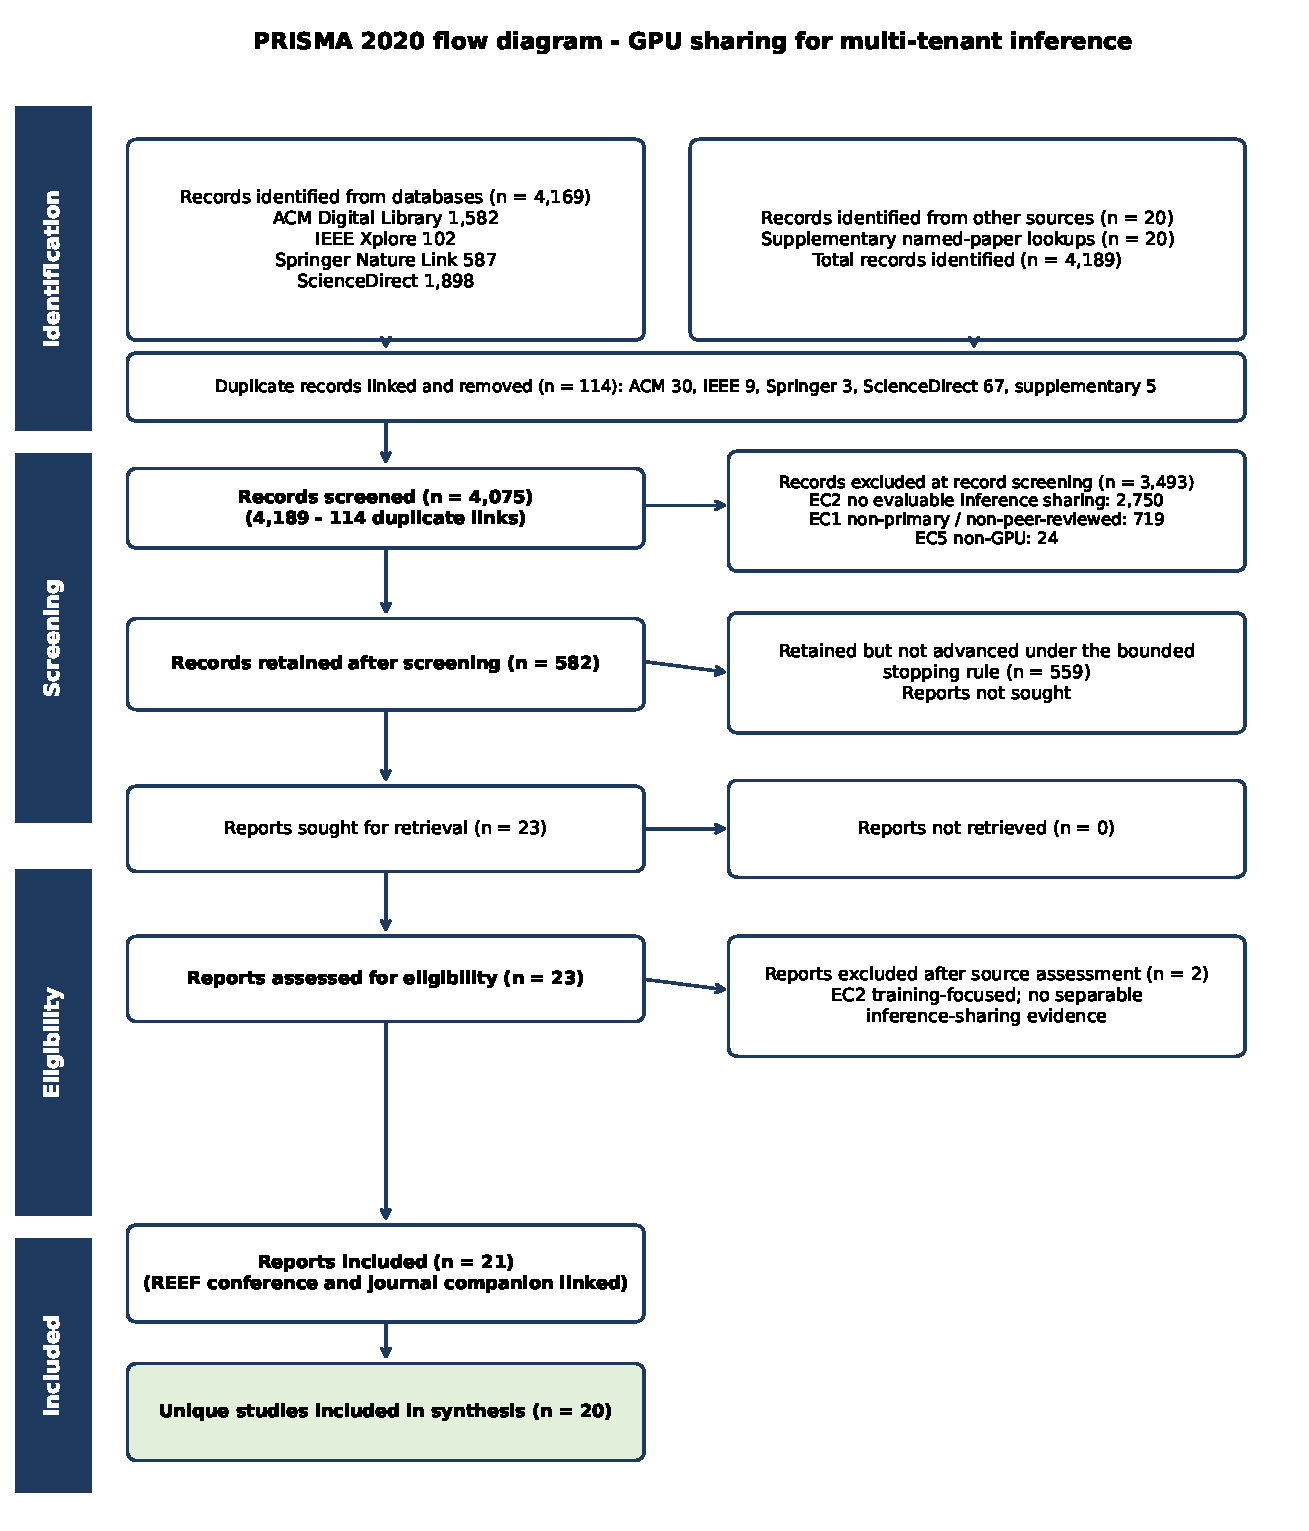
\includegraphics[width=\textwidth,height=.82\textheight,keepaspectratio]{../baseline/PRISMA_2020_FLOW_DIAGRAM.pdf}
\caption{Supplied bounded-review selection flow, preserved from Task 2. Current PDF download attempts are a separate activity.}
\end{figure}
\begin{longtable}{>{\raggedright\arraybackslash}p{0.16\textwidth}>{\raggedright\arraybackslash}p{0.62\textwidth}>{\raggedright\arraybackslash}p{0.1\textwidth}}
\toprule
\textbf{Study / report} & \textbf{System / source identity} & \textbf{QA}\\\midrule\endhead
S001 / P001 & VastPipe (2025) & 13/18\\\addlinespace
S002 / P002 & iGniter (2023) & 17/20\\\addlinespace
S003 / P003 & gpulets (2022) & 18/20\\\addlinespace
S004 / P004 & PipeSwitch (2020) & 17/20\\\addlinespace
S005 / P005 & REEF conference (2022) & 17/20\\\addlinespace
S006 / P006 & Paella: Low-latency Model Serving with Software-defined GPU Scheduling (2023) & 16/18\\\addlinespace
S007 / P007 & Orion: Interference-aware, Fine-grained GPU Sharing for ML Applications (2024) & 19/20\\\addlinespace
S008 / P008 & GSLICE: Controlled Spatial Sharing of GPUs for a Scalable Inference Platform (2020) & 17/20\\\addlinespace
S009 / P009 & Serving DNNs like Clockwork: Performance Predictability from the Bottom Up (2020) & 16/20\\\addlinespace
S010 / P010 & Colocating ML Inference and Training with Fast GPU Memory Handover (SIRIUS) (2025) & 17/20\\\addlinespace
S011 / P011 & ParvaGPU: Efficient Spatial GPU Sharing for Large-Scale DNN Inference in Cloud Environments (2024) & 14/20\\\addlinespace
S012 / P012 & Torpor: GPU-Enabled Serverless Computing for Low-Latency, Resource-Efficient Inference (2025) & 15/20\\\addlinespace
S013 / P013 & StreamBox: A Lightweight GPU SandBox for Serverless Inference Workflow (2024) & 15/20\\\addlinespace
S014 / P014 & Efficient Performance-Aware GPU Sharing with Compatibility and Isolation through Kernel Space Interception (KRYPTON) (2025) & 16/20\\\addlinespace
S015 / P015 & XSched: Preemptive Scheduling for Diverse XPUs (2025) & 16/18\\\addlinespace
S016 / P018 & InferFair: Towards QoS-aware scheduling for performance isolation guarantee in heterogeneous model serving systems (2024) & 15/20\\\addlinespace
S017 / P019 & ArkGPU: enabling applications' high-goodput co-location execution on multitasking GPUs (2023) & 16/20\\\addlinespace
S018 / P020 & Dyna-P: placement-aware dynamic partitioning for lightweight applications with modern GPUs (2025) & 15/20\\\addlinespace
S019 / P021 & KRISP: Enabling Kernel-wise RIght-sizing for Spatial Partitioned GPU Inference Servers (2023) & 16/20\\\addlinespace
S020 / P022 & Tally: Non-Intrusive Performance Isolation for Concurrent Deep Learning Workloads (2025) & 17/20\\\addlinespace
\bottomrule\end{longtable}

\section{Taxonomy of existing approaches}
A useful taxonomy separates the resource being controlled from the software layer implementing the policy. The same system may appear in more than one category. A MIG-based system can also use MPS; an API interceptor can enforce temporal scheduling; and memory handover can support mixed-workload co-location. Treating these as mutually exclusive labels would hide the source of the observed behavior.

\subsection{Temporal and priority control}
Temporal mechanisms decide which work runs and when another tenant can make progress. PipeSwitch emphasizes switching and model state, Clockwork emphasizes predictable execution and admission, while REEF, Paella, Orion and XSched expose different scheduling/preemption boundaries. Their integration costs and latency meanings differ. PipeSwitch's additional switching-related latency is not interchangeable with XSched's foreground P99 ratio or Paella's reported P99 reduction \cite{P004,P005,P006,P007,P009,P015}.

\subsection{Spatial allocation and partitions}
MPS-based allocation and software right-sizing regulate concurrent access to execution resources. VastPipe, iGniter, gpulets and GSLICE provide different allocation, profiling and feedback approaches. KRISP contributes AMD-oriented kernel right-sizing evidence and should not be relabeled as a measurement of NVIDIA MPS. Partition-aware designs, including ParvaGPU and Dyna-P, additionally make placement, profile size or reconfiguration relevant \cite{P001,P002,P003,P008,P011,P020,P021}.

A spatial allocation is only one part of a service guarantee. The model must fit memory, the workload must remain within the profiled regime and the selected resource shares must satisfy its timing requirements. Hardware allocation boundaries do not by themselves establish all possible security or fault guarantees in the reviewed experiments.

\subsection{API, runtime and memory mediation}
Torpor, StreamBox, KRYPTON, ArkGPU and Tally intervene at different points between the application and accelerator. Their common advantage is control over resource use without necessarily changing the model's high-level purpose. Their differences include intercepted interfaces, compatibility, runtime sharing, host work and the degree to which tenants share memory or trust assumptions. SIRIUS contributes a specific memory-handover mechanism for co-located inference and training \cite{P010,P012,P013,P014,P019,P022}.
\begin{longtable}{>{\raggedright\arraybackslash}p{0.25\textwidth}>{\raggedright\arraybackslash}p{0.35\textwidth}>{\raggedright\arraybackslash}p{0.28\textwidth}}
\toprule
\textbf{Family / reports} & \textbf{Control and condition} & \textbf{Cost}\\\midrule\endhead
Temporal / priority; P004 P005 P006 P007 P009 P015 P022 & Request, model, kernel or launch order. A suitable interception/preemption boundary exists & Switch cost, profiling and background slowdown\\\addlinespace
Software spatial sharing; P001 P002 P003 P008 P021 & MPS quota or AMD CU-mask control. Concurrent jobs fit memory and selected compute allocation & Residual interference; quotas are not proof of security\\\addlinespace
Hardware partition and hybrid; P011 P014 P020 & MIG profiles plus temporal/MPS policy. Supported partition profiles fit model memory & Fragmentation, placement and reconfiguration cost\\\addlinespace
API / runtime mediation; P006 P012 P013 P014 P019 P022 & User API, shared runtime or kernel interface. Required APIs and integration hooks are supported & Compatibility, CPU/transfer cost and trust boundary\\\addlinespace
Memory handover; P010 & Inference/training memory ownership. Training can yield memory without breaking inference & Reclamation and integration overhead\\\addlinespace
Fairness policy; P018 & Relative model slowdown and SLO goodput. Comparable per-model service objectives & Not equivalent to request-tail or hostile-tenant isolation\\\addlinespace
\bottomrule\end{longtable}

\section{Results and evidence synthesis by research question}
\subsection{RQ1: mechanisms and control boundaries}
The corpus supports a layered answer rather than a product list. Temporal control manages ordering and interruption; software spatial control manages concurrent allocation; hardware partitioning constrains resource placement; and API/runtime mediation supplies an enforcement layer. Fairness-aware policy adds a decision objective across these mechanisms. InferFair, for example, is best understood through relative slowdown and useful service, not as a new hardware partition primitive \cite{P018}.

This taxonomy explains why naming MPS, MIG or remoting is insufficient for engineering selection. A deployment also needs a policy, a mechanism for enforcing it and an explicit boundary of protection. The corpus demonstrates several combinations, but its bounded selection does not support a claim that one category is most prevalent in the entire literature.

\subsection{RQ2: measurements and comparability}
The outcome register includes requests/s, normalized throughput, goodput, P99/P98 latency, unspecified latency, SLO-violation rate, API overhead, host memory and a composite utilization-efficacy score. These measure different properties. Goodput counts work that meets a service objective, while aggregate throughput may include best-effort work that does not protect the foreground service. A numerical increase in the latter cannot establish improvement in the former.

GSLICE's GUE value of 94.04 is a composite score, not 94.04\% GPU utilization. Its negative signed latency improvement is retained as an unfavorable observation. The gpulets threshold covering 90\% of tested model pairs concerns a distribution across pairs, not the 90th percentile of requests. These distinctions prevent apparently precise but invalid conclusions \cite{P003,P008}.

The reported iGniter prediction-error range of 1.53--5.02\% assesses prediction accuracy, not a latency speedup. Clockwork's approximately 800 requests/s is goodput in a particular evaluation, and the supplied extraction notes a nonidentical comparator setup. Both observations are useful, but neither supports a direct ranking against a throughput ratio measured on another platform \cite{P002,P009}.

\subsection{RQ3: conditions affecting results}
Three conditions recur in the evidence. First, concurrency and resource shares affect both completed work and waiting time. The local ParvaGPU contrast shows a throughput benefit accompanied by increased latency. Second, model state and memory transfer can dominate. Torpor's late binding is attractive for low-rate functions, but its density result does not establish that frequent transfers of large models meet the same latency objective. Third, the workload's priority structure determines which sacrifice is acceptable \cite{P011,P012}.

For a foreground-priority service, XSched's 1.07x standalone P99 is relevant because it directly expresses foreground interference in the evaluated setup. Orion's up-to-7.3x aggregate-throughput result describes total work and must be read with its foreground-latency condition. These results can support different decisions without contradicting each other \cite{P007,P015}.

Mixed-workload evidence requires an additional separation. SIRIUS reports an average P99 inference improvement factor of 12.6 against the authors' adapted TaskSwitch baseline. It is not a uniform per-model gain or a direct comparison against unmodified PipeSwitch. ArkGPU's recorded inference/training pairs meet a twice-solo P99 target, while a low-contention setting can lose about 5\% QPS. The unfavorable condition belongs in the synthesis because it changes when the mechanism is worthwhile \cite{P010,P019}.

\subsection{RQ4: isolation and implementation cost}
Performance isolation asks whether another workload changes service behavior. Resource isolation asks what capacity is allocated or separated. Memory protection and fault containment concern different failure or adversarial models. A scheduler that limits slowdown is not thereby a complete hostile-tenant security boundary. The extraction cards preserve these dimensions separately, and untested boundaries remain unestablished.

Implementation costs also operate at different levels. API mediation can add host-side work or per-call delay. Model swapping adds transfer and memory pressure. Kernel-space interception introduces compatibility and maintenance requirements. Temporal granularity changes the trade-off between scheduling work and waiting time. The KRYPTON extraction reports an average QoS violation rate of 1.23\% relative to a solo P99 threshold, which is a threshold-relative request fraction rather than a latency in milliseconds. Its original Poisson rate is half the solo maximum; the shared test halves that rate again while assigning 50\% time \cite{P014}.

\subsection{RQ5: conditional selection}
The evidence supports a sequence of decisions. Specify the service objective and trust boundary first. Eliminate mechanisms incompatible with hardware, model memory or required integration. Compare the remaining candidates under the relevant arrival process, batch and co-tenant mix. Measure both protected service and work sacrificed. If the available studies do not cover the required boundary, the appropriate conclusion is insufficient evidence for that guarantee, not an assumed benefit.

The recommendation matrix in Section~10 connects each scenario to report IDs, expected benefits, costs and alternatives. These are evidence-supported candidates for evaluation, not claims that the reviewed implementation can be deployed unchanged in every environment.

\section{Comparative analysis}
The comparison distinguishes direct within-source contrasts from unmatched cross-study observations. The strongest numerical statements are tied to their original comparator. Even these require attention to whether the result is an average, maximum, lower bound or threshold-relative statistic. An improvement described as ``up to'' is not the expected result for an arbitrary deployment.

\begin{longtable}{>{\raggedright\arraybackslash}p{0.26\textwidth}>{\raggedright\arraybackslash}p{0.28\textwidth}>{\raggedright\arraybackslash}p{0.34\textwidth}}
\toprule
\textbf{Evidence / class} & \textbf{Observation} & \textbf{Interpretation and missing control}\\\midrule\endhead
CMP01 P011 E036 E037 C001 C002. Within-source trade-off & 354 to 446 requests/s; 11 to 27 ms & 25.99\% throughput increase accompanies 2.4545x latency. Missing: Latency quantile; final version equivalence\\\addlinespace
CMP02 P001 E001; P011 E036. Unmatched cross-study & 2.7x versus 25.99\% increase & Different baseline and GPU/model context prevent ranking. Missing: Matched workload, batch and resource budget\\\addlinespace
CMP03 P007 E029 E030; P015 E044. Different objectives & Up to 7.3x aggregate work versus 1.07x foreground P99 & Foreground delay and total completed work must be assessed together. Missing: Common model mix and background progress metric\\\addlinespace
CMP04 P008 E031 E032. Within-source metric tension & GUE 94.04 and negative signed latency improvement & Composite efficacy is not utilization percent; preserve adverse latency. Missing: Metric definitions and baseline stratum\\\addlinespace
CMP05 P012 E038 E039. Condition-dependent trade-off & Density benefit with model-transfer sensitivity & Late binding suits low-rate functions only if transfer fits SLO. Missing: Heavy-model transfer and host CPU budget\\\addlinespace
CMP06 P019 E048 E049; P022 E052. Different experiments, consistent cost & QoS protection with low-contention or background throughput loss & Protecting foreground work can sacrifice co-tenant work. Missing: Matched slowdown definitions\\\addlinespace
CMP07 P005 P023. Companion study, not replication & REEF engines and report versions differ & Retain source-version strata; do not double-count corroboration. Missing: Outcome-to-version mapping for every combined REEF row\\\addlinespace
CMP08 P018 E046 E047; P020 E050. Different metrics & Goodput/fairness versus makespan & Job-level efficiency cannot establish request-tail service. Missing: Request arrival process and latency distribution\\\addlinespace
\bottomrule\end{longtable}

The evidence table in Appendix~\ref{app:evidence} retains all 52 supplied observations. The comparative matrix is deliberately smaller because its role is to explain a decision, not duplicate the extraction register. A claim can be traced from a recommendation to a report, then to an outcome ID and its page/figure anchor. Where a comparison remains unmatched, the matrix names the missing control rather than calculating a misleading combined effect.

\section{Engineering trade-off analysis}
\subsection{Utilization versus latency}
Additional concurrency is beneficial only while useful service increases under the required latency objective. The ParvaGPU example changes throughput by
\[ (446/354-1)\times100 = 25.99\%, \]
while latency changes by
\[ 27/11 = 2.4545. \]
These are calculations from recorded inputs, not newly measured outcomes. A service with a tight delay budget might reject this configuration despite its higher throughput. Another service might accept it if the increased latency remains within its own budget. Because the source quantile is unspecified, neither interpretation establishes P99 compliance \cite{P011}.

\subsection{Foreground protection versus background progress}
Priority is an allocation choice. Tally's supplied contrast records normalized background throughput of 1.19 versus 1.65 for TGS at the stated idle-time setting. This does not make foreground protection ineffective; it identifies the work sacrificed. Similarly, an aggregate-throughput gain must not hide deterioration in the protected request class. The engineering evaluation should report foreground latency and background progress together \cite{P022}.

\subsection{Memory density versus transfer and trust costs}
Shared runtimes and late binding can allow more functions or models to use limited GPU memory. StreamBox's workflow-oriented sharing and Torpor's binding decisions address this problem from different directions. Their density gains cannot be separated from concurrency, model-loading and trust assumptions. When large models are invoked frequently, transfer demand can undermine the benefit of keeping fewer models resident. When functions require stronger separation, a shared runtime may not provide the required boundary. Torpor explicitly distinguishes runtime-sharing evaluation from runtime-isolation deployment, and describes restart/migration recovery; these design claims are not direct fault-injection results \cite{P012,P013}.

\subsection{Partition control versus flexibility}
Hardware profiles constrain placement and memory fit. Software policies can improve use of a chosen profile, but fine-grained application demand need not align with fixed partitions. Dyna-P's recorded sensitivity to prediction perturbation concerns makespan, while online serving additionally needs evidence about individual request delays. The review therefore treats placement efficiency as relevant but insufficient evidence for latency-sensitive request serving \cite{P020}.

\section{Discussion and conflicting evidence}
\subsection{Apparent conflicts versus controlled disagreements}
A valid conflicting-evidence analysis first asks whether two studies measure the same quantity under comparable conditions. VastPipe's 2.7x throughput contrast and the calculated 25.99\% ParvaGPU increase have different baselines and workloads. Their unequal magnitudes do not show disagreement. Likewise, Orion's aggregate throughput, SIRIUS's average P99 improvement and XSched's normalized foreground P99 do not compete on a common scale \cite{P001,P007,P010,P011,P015}.

More useful tensions occur inside an experiment: improved throughput accompanied by higher latency, or protection of foreground work accompanied by lower background progress. The negative GSLICE latency contrast and ArkGPU's low-contention regression show conditions in which a favorable overall mechanism narrative is incomplete. These observations constrain applicability rather than being dismissed as exceptions \cite{P008,P019}.

\subsection{Version and engine effects}
The REEF journal extension adds implementation and evaluation beyond the conference report. The supplied extraction already distinguishes PyTorch and TensorRT conditions in its discussion. Combining all favorable points into one synthetic result would obscure both the engine difference and the report-version difference. The current study-level mapping avoids double-counting, but each combined REEF outcome still needs an explicit conference-versus-journal source assignment before final submission \cite{P005,P023}.

\subsection{Strength of the engineering argument}
The repeated pattern is that resource sharing works through a mechanism-specific constraint: interruption cost, quota fit, memory residency, partition placement or compatibility. This pattern supports conditional design reasoning. It does not establish identical effect sizes or a common security guarantee across systems. The draft's recommendations remain narrower than a claim of deployment readiness.

\section{Evidence-based engineering recommendations}
\subsubsection*{REC01: Trusted resident models; utilization priority}
\begin{longtable}{>{\raggedright\arraybackslash}p{0.22\textwidth}>{\raggedright\arraybackslash}p{0.7\textwidth}}
\toprule
\textbf{Dimension} & \textbf{Assessment}\\\midrule\endhead
Candidate & Tuned MPS / software spatial controls\\\addlinespace
Evidence & P001 P002 P003 P008 E001-E004 E006 E031-E032\\\addlinespace
Expected benefit & Higher useful co-location under tested allocations\\\addlinespace
Sacrifice & Interference, quota tuning and memory pressure\\\addlinespace
Alternative / trigger & Partitions or dedication when trust/isolation dominates\\\addlinespace
Validation needed & Measure each model P99 and SLO goodput under bursts\\\addlinespace
\bottomrule\end{longtable}
\subsubsection*{REC02: Foreground tail-latency priority}
\begin{longtable}{>{\raggedright\arraybackslash}p{0.22\textwidth}>{\raggedright\arraybackslash}p{0.7\textwidth}}
\toprule
\textbf{Dimension} & \textbf{Assessment}\\\midrule\endhead
Candidate & Priority/preemptive scheduling\\\addlinespace
Evidence & P005 P006 P007 P015 P022 E018-E030 E044-E045 E052\\\addlinespace
Expected benefit & Lower foreground interference\\\addlinespace
Sacrifice & Background slowdown, profiling and runtime integration\\\addlinespace
Alternative / trigger & Dedicated GPU when supported control cannot meet deadline\\\addlinespace
Validation needed & Check foreground tails and background progress jointly\\\addlinespace
\bottomrule\end{longtable}
\subsubsection*{REC03: Low-rate serverless functions}
\begin{longtable}{>{\raggedright\arraybackslash}p{0.22\textwidth}>{\raggedright\arraybackslash}p{0.7\textwidth}}
\toprule
\textbf{Dimension} & \textbf{Assessment}\\\midrule\endhead
Candidate & Late binding / controlled runtime sharing\\\addlinespace
Evidence & P012 P013 E038-E041\\\addlinespace
Expected benefit & Higher function or workflow density\\\addlinespace
Sacrifice & Host CPU, memory transfer and shared-runtime trust\\\addlinespace
Alternative / trigger & Keep large or high-rate models resident if swaps dominate\\\addlinespace
Validation needed & Sweep model sizes, cold starts, offered rate and concurrency\\\addlinespace
\bottomrule\end{longtable}
\subsubsection*{REC04: Mixed inference with opportunistic training}
\begin{longtable}{>{\raggedright\arraybackslash}p{0.22\textwidth}>{\raggedright\arraybackslash}p{0.7\textwidth}}
\toprule
\textbf{Dimension} & \textbf{Assessment}\\\midrule\endhead
Candidate & Memory handover / controlled co-location\\\addlinespace
Evidence & P010 P019 E035 E048-E049\\\addlinespace
Expected benefit & Protect inference while using residual capacity\\\addlinespace
Sacrifice & Reclamation overhead and reduced training progress\\\addlinespace
Alternative / trigger & Separate resources for intolerable interference\\\addlinespace
Validation needed & Measure inference tails separately from training throughput\\\addlinespace
\bottomrule\end{longtable}
\subsubsection*{REC05: Supported partition hardware; stable memory fit}
\begin{longtable}{>{\raggedright\arraybackslash}p{0.22\textwidth}>{\raggedright\arraybackslash}p{0.7\textwidth}}
\toprule
\textbf{Dimension} & \textbf{Assessment}\\\midrule\endhead
Candidate & MIG-aware hybrid policy\\\addlinespace
Evidence & P011 P014 P020 E036-E037 E042-E043 E050\\\addlinespace
Expected benefit & Resource allocation with configurable co-location\\\addlinespace
Sacrifice & Fragmentation and reconfiguration overhead\\\addlinespace
Alternative / trigger & Software sharing when partition granularity wastes capacity\\\addlinespace
Validation needed & Validate profile fit and reconfiguration effects; security needs separate tests\\\addlinespace
\bottomrule\end{longtable}
\subsubsection*{REC06: Several models with unequal service pressure}
\begin{longtable}{>{\raggedright\arraybackslash}p{0.22\textwidth}>{\raggedright\arraybackslash}p{0.7\textwidth}}
\toprule
\textbf{Dimension} & \textbf{Assessment}\\\midrule\endhead
Candidate & Fairness-aware admission / scheduling\\\addlinespace
Evidence & P018 E046-E047\\\addlinespace
Expected benefit & Balance normalized slowdown and SLO goodput\\\addlinespace
Sacrifice & May give up aggregate throughput to improve fairness\\\addlinespace
Alternative / trigger & Priority scheduling when one foreground SLA dominates\\\addlinespace
Validation needed & Agree fairness objective and per-model SLO before deployment\\\addlinespace
\bottomrule\end{longtable}
The recommended deployment assessment begins with the actual service objective: per-model deadline or percentile target, admissible violation rate and minimum background progress. These values must come from the intended deployment rather than being invented from a paper. The next step is a local comparison using the same model versions, input sizes, batching and offered load. Cold starts and bursts should be retained if they occur in the application.

A candidate is suitable only if it meets the required service objective at an acceptable cost. The acceptance evidence should include per-tenant latency, SLO-compliant goodput, memory pressure, resource utilization with a defined instrument, host overhead and the relevant isolation tests. The review supplies a shortlist and the reasons to test it; it does not supply a universal numerical threshold or imply that a benchmark result transfers unchanged.

\section{Research gaps and future directions}
\begin{longtable}{>{\raggedright\arraybackslash}p{0.28\textwidth}>{\raggedright\arraybackslash}p{0.22\textwidth}>{\raggedright\arraybackslash}p{0.38\textwidth}}
\toprule
\textbf{Corpus gap} & \textbf{Basis} & \textbf{Next experiment}\\\midrule\endhead
No matched all-family comparison & Comparability CMP01-CMP08 & Same GPU, model mix, memory budget, arrivals and SLO across families\\\addlinespace
Security/fault boundaries often unestablished & Extraction Security boundary / Fault boundary & Separate adversarial access, fault injection and performance tests\\\addlinespace
Metrics emphasize different units & E001-E052 & Report per-model goodput, tails and background progress jointly\\\addlinespace
Partition prediction affects makespan & P020 E050 & Bursty arrivals plus placement changes and request-tail measurement\\\addlinespace
Version and method details remain incomplete & P002 P011 P022; QA Q3/Q4/Q10 & Publish exact version, driver/runtime, warmup, repetitions and uncertainty\\\addlinespace
Energy and cost evidence not harmonized & Extraction schema and heterogeneous outcomes & Measure GPU and host energy per SLO-compliant request\\\addlinespace
\bottomrule\end{longtable}
These gaps are observations about this corpus and its reporting, not assertions that no relevant research exists anywhere. The 559-record unassessed branch makes that distinction essential. A stronger future comparison would align hardware, workload, baselines and outcome definitions across mechanism families, then report both benefits and sacrifices. Energy per useful request and failure/security behavior require separate measurements rather than extrapolation from utilization.

\section{Threats to validity and limitations}
\begin{longtable}{>{\raggedright\arraybackslash}p{0.32\textwidth}>{\raggedright\arraybackslash}p{0.26\textwidth}>{\raggedright\arraybackslash}p{0.3\textwidth}}
\toprule
\textbf{Threat / consequence} & \textbf{Mitigation} & \textbf{Remaining work}\\\midrule\endhead
Selection/stopping: No exhaustive recall or prevalence claim & Stopping branch remains visible & Instructor/team decision on bounded scope; extend if required\\\addlinespace
Title-only decisions: Relevant work may be missed & Abstract-availability column retained & Prioritize uncertain/relevant records for abstract checks\\\addlinespace
Single review: Correlated screening/QA/extraction errors possible & Original rationale and source anchors retained & Record real named checks if performed\\\addlinespace
Search provenance: Search cannot be fully reconstructed from totals & Exact preserved query/log values retained & Supply missing original exports, facets and receipts\\\addlinespace
Source version: Page/result mappings may differ & Separate source-version and retrieval records & Compare final published text and map companion outcomes\\\addlinespace
Measurement heterogeneity: Cross-study speedup ranking is invalid & No pooled effect size or universal winner & Matched comparisons needed\\\addlinespace
Reporting bias: Headlines may overstate robustness & Adverse and null findings retained & Recheck high-impact claims at exact source locations\\\addlinespace
\bottomrule\end{longtable}
The most material limitation is selection: a bounded source set cannot establish exhaustive coverage. The large number of title-only records compounds that risk. The single-assessment method creates a separate risk of correlated errors even where spreadsheet arithmetic is correct. Finally, retrieved author manuscripts may differ from the version used by the original extraction, and access to a PDF does not constitute verification of every result.

Mitigations in this draft include immutable baseline files, separate current retrieval records, stable IDs, preserved unfavorable findings, explicit source/version limits and no numerical pooling across unmatched studies. These measures improve traceability but do not erase the underlying limitations. Final acceptance requires resolving the scope decision and recording any actual independent checks at the item level.

\section{Conclusion}
The bounded 20-study corpus supports a conditional approach to GPU sharing for multi-tenant inference. Temporal control is relevant when foreground response dominates; software spatial sharing is relevant when trusted co-location can exploit spare capacity; partition-aware designs make resource fit and reconfiguration central; and runtime or memory mediation can increase density at a transfer, integration or trust cost. Each choice must be evaluated against its own baseline and intended conditions.

The principal outcome is therefore a traceable selection framework, not a universal ranking. The first draft covers the instructor's analytical requirements through Section 22 and follows the suggested final-report sequence. It remains a draft: the bounded scope, source-version mappings, incomplete PDF collection and item-level checking require explicit closure before the work is represented as a fully verified final SLR.
